% !TeX spellcheck = en_GB
\documentclass[11pt]{article}

\usepackage[type1]{libertine}
\usepackage[a4paper]{geometry}
\usepackage{amsmath, amsthm, amssymb} 
\usepackage{parskip}
\usepackage{tabularx}
\usepackage[english]{babel}
\usepackage{enumitem}
\usepackage{gensymb}
\usepackage{bm}
\usepackage{graphicx}
\usepackage{xcolor}
\usepackage{wrapfig}
\usepackage[makeroom]{cancel}
\usepackage{multicol}

\newcommand{\uvec}[1]{\boldsymbol{\hat{\textbf{#1}}}}

\title{Kinematics Tutorial 2B Worked Solutions}
\author{Sun Yudong\\Hwa Chong Institution}

\begin{document}
	\maketitle
	This only contains the solutions to the discussion questions of Tutorial 2B.
	\begin{enumerate}
		\item[{[D1]}] Let $\vec{u_x}$ be the horizontal velocity, and $\vec{S_x}$ and $\vec{S_y}$ be the horizontal and vertical displacement respectively.
			\begin{align*}
				\vec{S_y} = \frac{1}{2}~g\left(\frac{|\vec{S_x}|}{|\vec{u_x}|}\right)^2&=\left[\frac{1}{2}~g\frac{1}{|\vec{u_x}|^2}\right] |\vec{S_x}|^2 \\
				\implies \vec{S_y} &\propto |\vec{S_x}|^2 \\
				\frac{|\vec{S_{y_{_1}}}|}{|\vec{S_{x_{_1}}}|^2} &= \frac{|\vec{S_{y_{_2}}}|}{|\vec{S_{x_{_2}}}|^2} \\
				\therefore |\vec{S_{y_{_2}}}| &= \frac{|\vec{S_{y_{_1}}}|}{|\vec{S_{x_{_1}}}|^2} \times |\vec{S_{x_{_2}}}|^2 \\
				&= \frac{5.0 \text{mm}}{(25 \text{m})^2} \times (50 \text{m})^2 \\
				&= 20 \text{mm}
			\end{align*}
			
		\vfill
		\item[{[D2]}] Since $\displaystyle \theta = \tan^{-1}\left(\frac{v_x}{v_y}\right)$, we need to maximize $\displaystyle \frac{v_x}{v_y}$ to maximize $\theta$. \\ Since $v_x = v;~ v_y \propto \sqrt{h}$, we choose the smallest $v$ and the largest $h$ \\ $\implies$Option B.
		
		\vfill
		
		\item[{[D3]}] Draw vertical lines and horizontal lines through all the dots. The horizontal velocity (horizontal spacing) of the ball should remain constant, while the vertical velocity (vertical spacing) of the ball should increase at an increasing rate. This is because there is only gravitational force acting on the ball, and the gravitational force only affects the vertical velocity of the ball. \\ $\implies$ Option C
		
		\vfill
		
		\pagebreak
		
		\item[{[D4]}]
			Height is determined only by the vertical component of the initial velocity. The time of flight is given by how long it takes the ball to go up and then come down, and is not affected by horizontal velocity (since there are no horizontal obstacles).
			
			Given the same time of flight, the range is determined by how fast the ball is going horizontally, since the faster you go, the more distance you can cover within the same timeframe.
			\begin{multicols}{4}
				\begin{enumerate}		
					\item $a=b=c$
					\item $a=b=c$
					\item $a < b < c$
					\item $a < b < c$
				\end{enumerate}
			\end{multicols}
		
		\item[{[D5]}] We take $\rightarrow$ and $\uparrow$ as positive.
		\begin{align*}
			u_x &= \frac{60}{3.0} = 20 \text{ms}^{-1} \\
			s_y &= u_yt+\frac{1}{2}gt^2 \\
			15 &= u_y(3.0) + \frac{1}{2}(9.81)(3.0)^2 \\
			\implies u_y &= 9.715 \text{ms}^{-1}
		\end{align*}
		\begin{enumerate}
			\item $\displaystyle \theta = \tan^{-1}\left(\frac{9.715}{20}\right)=25.9 \degree$
			\item Speed $=\sqrt{u_y^2+u_x^2}=22.2\text{ms}^{-1}$
			\begin{align*}
				v_y^2=u_y^2+2gs \implies v_y &= \pm \sqrt{9.715^2+2(-9.81)(-15)} \\
				&=-19.715 ~~~\text{(}\because v_y ~\text{must be in the negative direction)}
			\end{align*}
			\item $\displaystyle \theta = \tan^{-1}\left(\frac{-19.715}{20}\right)=-44.6 \degree$
			\begin{figure}[h]
				\centering
				\def\svgwidth{3.5cm}
				\input{D5.pdf_tex}
			\end{figure}
			\item Speed $=\sqrt{v_y^2+v_x^2}=28.1~\text{ms}^{-1}$
		\end{enumerate}
		\pagebreak
		
		\item[{[D6]}] We take $\rightarrow$ and $\uparrow$ as positive.
		
		\begin{figure}[h!]
			\centering
			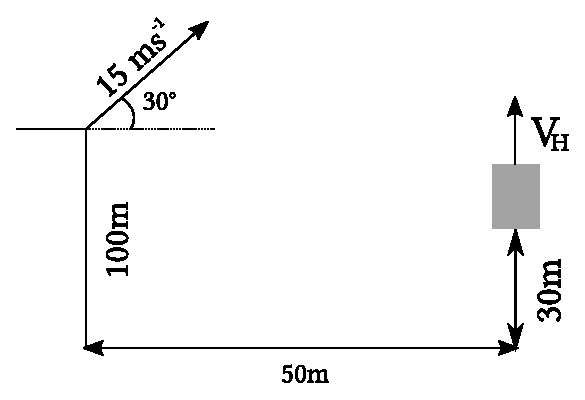
\includegraphics[width=0.5\columnwidth]{D6.eps}
		\end{figure}
		\begin{align*}
		\text{Total time taken} &= \frac{50}{15.0\cos(30\degree)} = 3.849 \text{s}\\
		S_{c_y} &= 15.0sin(30\degree)(3.849)+\frac{1}{2}(-9.81)(3.849)^2 \\ &= -43.79 \text{m} \\
		\therefore \text{Distance travelled by balloon} &= (100-30)-43.79 = 26.9\text{m} \\
		\therefore v_H &= \frac{26.2}{3.849} = 6.8 \text{ms}^{-1}
		\end{align*}
		\vfill
		\item [{[D7]}]
		\begin{enumerate}
			\item At the start of projection of the 2\textsuperscript{nd} ball. (Refer to answer for D3)
			\item Yes. Vertical velocity of Ball 1 is always larger than vertical velocity of Ball 2. Horizontal velocity of both balls are the same. Resultant velocity of Ball 1 is thus always greater.
			\item 1 s. They have the same trajectory. 
			\item No. Flight time is determined by the vertical velocity only.
		\end{enumerate}
		\vfill
		\pagebreak
		
		\item [{[D8]}]
		\begin{enumerate}[label=(\roman*)]
			\item $S_x = u\cos\theta t = 10\cos(60\degree) t = 5t$ \\ 
			$S_y = u\sin\theta t - \frac{1}{2}gt^2 = 10\sin(60\degree) t - \frac{1}{2}(9.81)t^2 = 5\sqrt{3}t - 4.905t^2$
			\item
			\begin{align*}
				-45\degree &= \arctan\left(\frac{S_y}{S_x}\right) \\
				\therefore S_y &= -S_x \\
				u\sin\theta t - \frac{1}{2}gt^2 &= -\left[u\cos\theta t\right] \\
				\frac{1}{2}gt^2 - u(\sin\theta-\cos\theta)t&= 0 \\
				t\left[\frac{1}{2}gt-u(\sin\theta-\cos\theta)\right] &= 0 \\
				\because t \neq 0 \therefore t &= \frac{2u(\sin\theta-\cos\theta)}{g}\\	
				&= \frac{2(10)(\sin60\degree -\cos60\degree)}{9.81} \\
				&= 2.78\text{s}
			\end{align*}
			\item 
			\begin{align*}
			d = \sqrt{S_x^2 + S_y^2} &= \sqrt{2}S_x \\
			&= 5\sqrt{2}\left(\frac{2(10)(\sin60\degree -\cos60\degree)}{9.81}\right) \\
			&=19.7 \text{m}
			\end{align*}
		\end{enumerate}
		
		\item [{[D9]}] We take $\downarrow$ and $\rightarrow$ as positive. Let $D$ be the distance between the points of impact of P and Q.
		\begin{align*}
			h &= u(\sin\theta)t_q + \frac{1}{2}gt_q^2 \\
			h &= -u(\sin\theta)t_p + \frac{1}{2}gt_p^2 \\
			D &= (t_p-t_q)u\cos\theta 
		\end{align*}
		Equating the first two equations:
		\begin{align*}
			u(\sin\theta)t_q + \frac{1}{2}gt_q^2 &= -u(\sin\theta)t_p + \frac{1}{2}(9.81)t_p^2 \\
			u(\sin\theta)\cancel{(t_p+t_q)} &= \frac{1}{2}g(t_p^2+t_q^2) \\
			&=\frac{1}{2}g\cancel{(t_p+t_q)}(t_p-t_q) \\
			D=(t_p-t_q)u\cos\theta  &= \frac{2u\sin\theta}{g}u\cos\theta \\
			&= \frac{u^2(2\sin\theta\cos\theta)}{g} \\
			&= \frac{u^2\sin(2\theta)}{g}
		\end{align*}
	\end{enumerate}
	
\end{document}